

%%%%%%%%%
%% Measurement Methodology 
\section{Measurement Methodology}
\label{sec:method}
Our measurements are conducted on the current POWDER deployment
on the University of Utah campus (Fig.~\ref{powdernodes}).
Part of the area includes a typical spread out university campus, while other parts
include a more densely populated urban-like environment. POWDER offers nine general purpose rooftop base stations that include networked software-defined-radios (SDRs), an RF front-end (frequency division duplex), and signal amplification. Furthermore, POWDER offers 10 fixed endpoints. 
Similar to the general purpose rooftop base stations, the components include SDRs, RF front-end and antenna elements. 

\subsection{Measurement Tool: Shout}
Shout is a measurements framework developed by the POWDER team~\cite{b2}. Using Shout you are able to collect RF
measurements for the nodes within the testbed. The framework was developed in Python and offers a rich set of measurement
collections. Shout follows a client-server architecture in which we have an orchestrator node running at all times. Each client 
radio node connects to the orchestrator via the POWDER control/out-of-band network. 

For our purposes we used Shout to collect RF propagation among the nodes on the platform. Shout uses JSON files as 
command files to tell the orchestrator how it should direct the other nodes. We used a configuration file which directed the
framework to treat each node as a receiver and transmitter in a round-robin fashion. The JSON file used follows this approach:
\begin{equation}
PL_M = CF + \frac{1}{2}SR\label{eq5}
\end{equation}
Where $CF$ is the center frequency (tuned frequency) and $SR$ is the sample rate. $PL_M$ describes the upper bound for
collection, with a frequency step size dictated by the JSON file. In other words for the given $CF$ we collect measurements 
up to $PL_M$ with a given frequency step. Shout then averages these results to produce an average received power for the
given frequency between two nodes. This is the approach we follow when calculating RF propagation using the Shout framework.

\subsection{Measurement Tool: SPLAT!}
SPLAT! will be our modeling tool to compare with Shout's results~\cite{b3}. SPLAT! can be used to produce terrain analysis 
maps of the designated area, but for our purposes we will use the SPLAT! point-to-point analysis model to calculate RF 
propagation. For RF propagation, SPLAT! requires two primary files: QTH, and LRP. QTH files are site location files that contain
the site's name, the site's latitude, the site's longitude and the site's antenna height above ground level. LRP files are the irregular
terrain model parameter files that are used to determine radio frequency path loss, field strength, or received signal power level. 

\begin{figure}[htbp]
\centerline{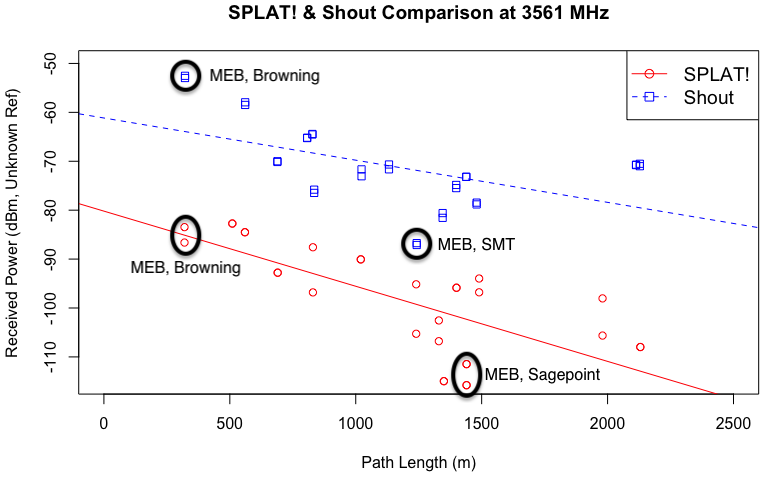
\includegraphics[width=0.9\columnwidth]{figs/3561.png}}
\vspace{-3mm}
\caption{Run 1. Used 3561 MHz frequency.}
\label{3561}
\vspace{-3mm}
\end{figure}

\begin{table}[htbp]
\caption{Path Loss Exponents for each run}
\begin{center}
\begin{tabular}{|c|c|c|c|}
\hline
\textbf{Run \#} & \textbf{\textit{Frequency (MHz)}}& \textbf{\textit{Shout (dBm/m)}}& \textbf{\textit{SPLAT! (dBm/m)}} \\
\hline
Run 1& $3561$& $-0.0086$& $-0.0154$  \\
Run 2& $2620$& $-0.0114$& $-0.0186$  \\
Run 3& $3550$& $-0.0132$& $-0.0113$  \\
Run 4& $3690$& $-0.0163$& $-0.0103$  \\
\hline
\end{tabular}
\label{tab1}
\vspace{-3mm}
\end{center}
\end{table}

To produce and compare accurate results between Shout and SPLAT!, we followed the same approach as in formula \eqref{eq5}. Using the 
proper QTH and LRP files for each node we created a Python script that easily mediates the process of collecting the data
for a given frequency. SPLAT! is a command-line driven application that reads in the data from the QTH and LRP files and produces a 
results file that can be parsed for the necessary data. 


\subsection{Measurements}
Following the above methodology we perform extensive measurements on the POWDER platform using Shout and SPLAT! using
multiple frequencies and nodes. For this effort we conducted four measurement runs with each run being done three times. These measurement runs span three different frequency ranges. To summarize: 
\begin{itemize}
\item Run 1 took place in early October. The measurement conducted used the 3561 MHz frequency, and used the: Behavioral 
Science, Browning, Friendship Manor, Sagepoint, MEB, and South Medical Tower nodes. This run was conducted at mid-day. 
\item Run 2 took place in early November. The measurement conducted used the 2620 MHz frequency, and used the: Behavioral
Science, Browning, Friendship Manor, Honors, Sagepoint, Ustar as transmitters nodes. And used Bookstore, EBC, Garage, 
Guesthouse, Humanities, Law73, Madsen, Moran, and WEB as receiver fixed endpoint nodes. This run does not follow the 
typical round-robin approach among all the nodes where each one acts as a receiver and transmitter because only the transmitter
nodes listed where able to transmit at the listed frequency. We still followed the approach discussed in equation~\eqref{eq5}.  This run was
conducted early morning. 
\item Run 3 took place in late November. The measurement conducted used the 3550 MHz frequency, and used the: Behavioral
Science, Browning, Honors, Sagepoint, South 

\begin{figure}[htbp]
\centerline{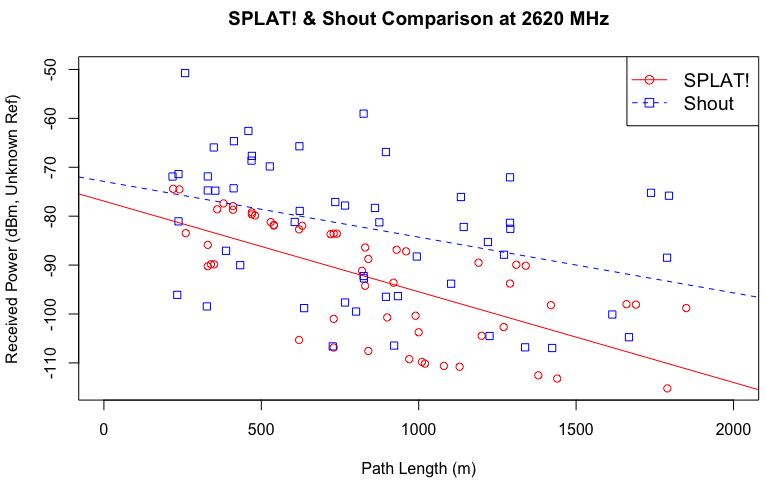
\includegraphics[width=0.9\columnwidth]{figs/2620.png}}
\vspace{-3mm}
\caption{Run 2. Used 2620 MHz frequency.}
\label{2620}
\vspace{-3mm}
\end{figure}

Medical Tower, Ustar, and Friendship Manor nodes. This run was conducted early 
morning. 
\item Run 4 took place in late November. The measurement conducted used the 3690 MHz frequency, and used the: Behavioral 
Science, Browning, Honors, Sagepoint, South Medical Tower, Ustar, and Friendship Manor nodes. This run was conducted early 
morning.
\end{itemize}


